\documentclass[tikz]{standalone}

\begin{document}
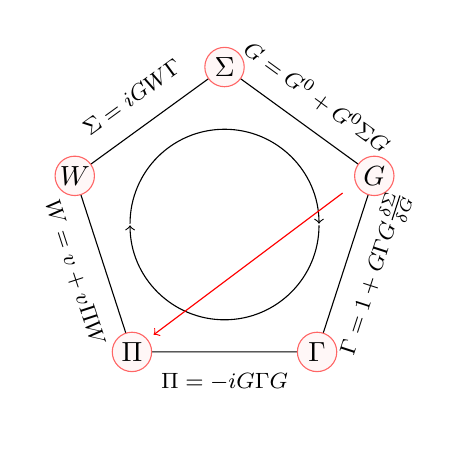
\begin{tikzpicture}
\clip (-2.5, -2.5) rectangle (2.5,2.5);
	
\draw (0,2) -- (-1.90211,0.618) -- (-1.17557,-1.618) -- (1.17557,-1.618) -- (1.90211,0.618)--cycle;:

\filldraw[color=red!60, fill=red!3](0,2) circle (0.25);
\node[] at (0, 2) {$\Sigma$};

\filldraw[color=red!60, fill=red!3](-1.90211,0.618) circle (0.25);
\node[] at (-1.90211,0.618) {$W$};

\filldraw[color=red!60, fill=red!3](-1.17557,-1.618) circle (0.25);
\node[] at (-1.17557,-1.618) {$\Pi$};

\filldraw[color=red!60, fill=red!3](1.17557,-1.618) circle (0.25);
\node[] at (1.17557,-1.618) {$\Gamma$};

\filldraw[color=red!60, fill=red!3](1.90211,0.618) circle (0.25);
\node[] at (1.90211,0.618) {$G$};


\node[rotate=36] at (-1.17557,1.618) {\footnotesize $\Sigma=iGW\Gamma$};
\node[rotate=-36] at (1.17557,1.618) {\footnotesize $G=G^0+G^0\Sigma G$};
\node[rotate=-72] at (-1.90211,-0.618) {\footnotesize $W=v+v\Pi W$};
\node[rotate=72] at (1.90211,-0.618) {\footnotesize $\Gamma=1+G\Gamma G\frac{\delta \Sigma}{\delta G}$};

\node[rotate=0] at (0,-2) {\footnotesize $\Pi = -iG\Gamma G$};

\draw[->] (1.2,-0.01) arc (0:-180:1.2);
\draw[->] (-1.2,0.01) arc (180:0:1.2);

\draw[red, ->] (1.5,0.4) -- (-0.9,-1.4);



\end{tikzpicture}
\end{document}
